% Chapter Template

\chapter{Resultados} % Main chapter title

\label{Chapter4} % Change X to a consecutive number; for referencing this chapter elsewhere, use \ref{ChapterX}

\lhead{Capítulo 4. \emph{Resultados}} % Change X to a consecutive number; this is for the header on each page - perhaps a shortened title

\section{Resultados de Rendimiento}

\subsection{Tiempos de carga}
TODO: Cuadro con los tiempos de carga de una escena con un numero variable de modelos
\subsection{Renderizado de Múltiples Objetos Simples}
Se ha decidido comprobar el rendimiento de \robotto al renderizar múltiples objetos simples, es decir, objetos carentes de texturas o animaciones.\\
Todos estos objetos son individuales, es decir, aunque se vean iguales cada uno posee una malla diferente asociada.\\

\begin{table}[h]
\centering
\caption{My caption}
\label{my-label}
\begin{tabular}{|l|l|l|l|l|l|}
\hline
Nº de objetos & 5  & 10 & 20 & 50 & 80 \\ \hline
FPS           & 60 & 60 & 59 & 45 & 28 \\ \hline
\end{tabular}
\end{table}

\begin{figure}[h!]
\centering
\subfloat[5 objetos]{
  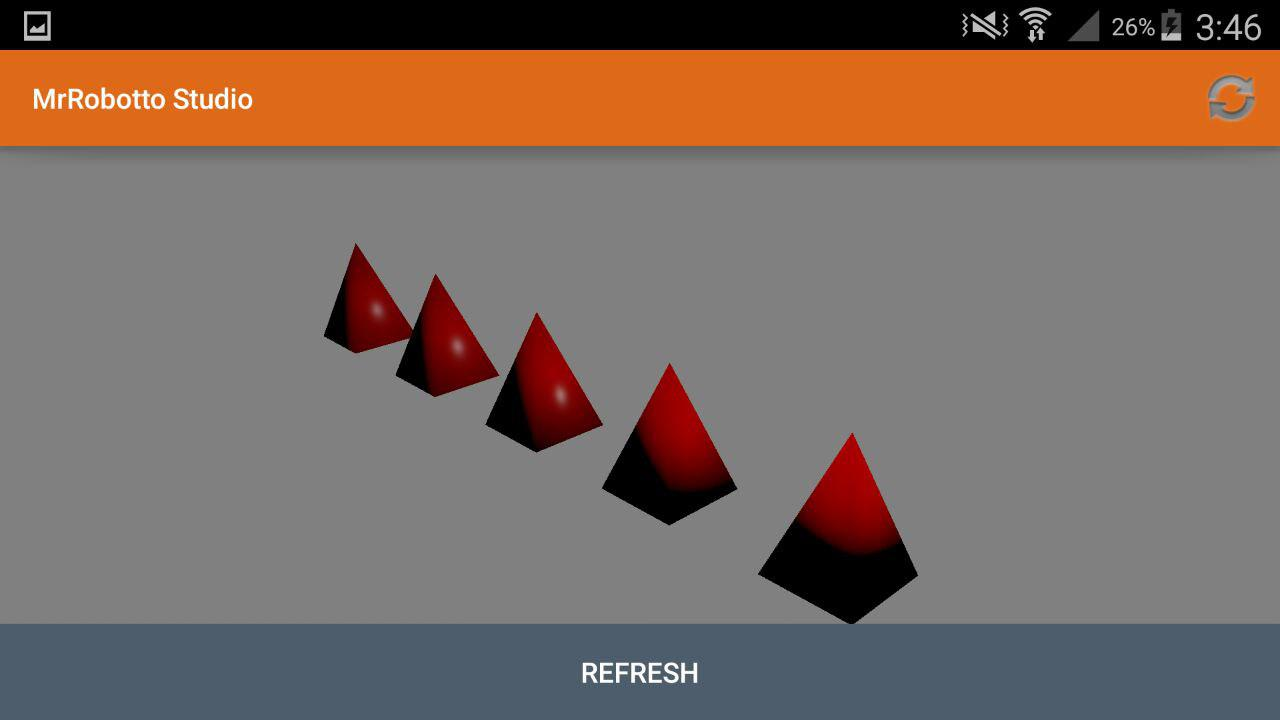
\includegraphics[scale=0.1]{benchmarks/simple/5.jpg}
}
\subfloat[10 objetos]{
  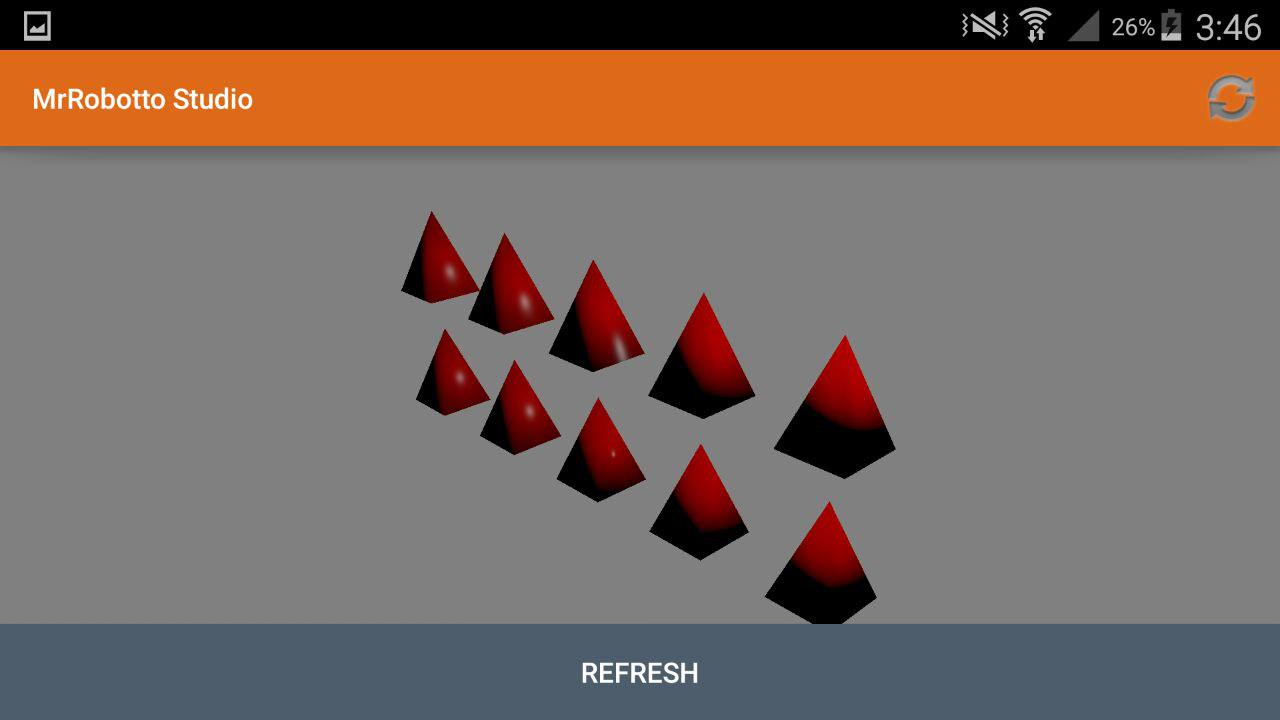
\includegraphics[scale=0.1]{benchmarks/simple/10.jpg}
}
\hspace{0mm}
\subfloat[20 objetos]{
  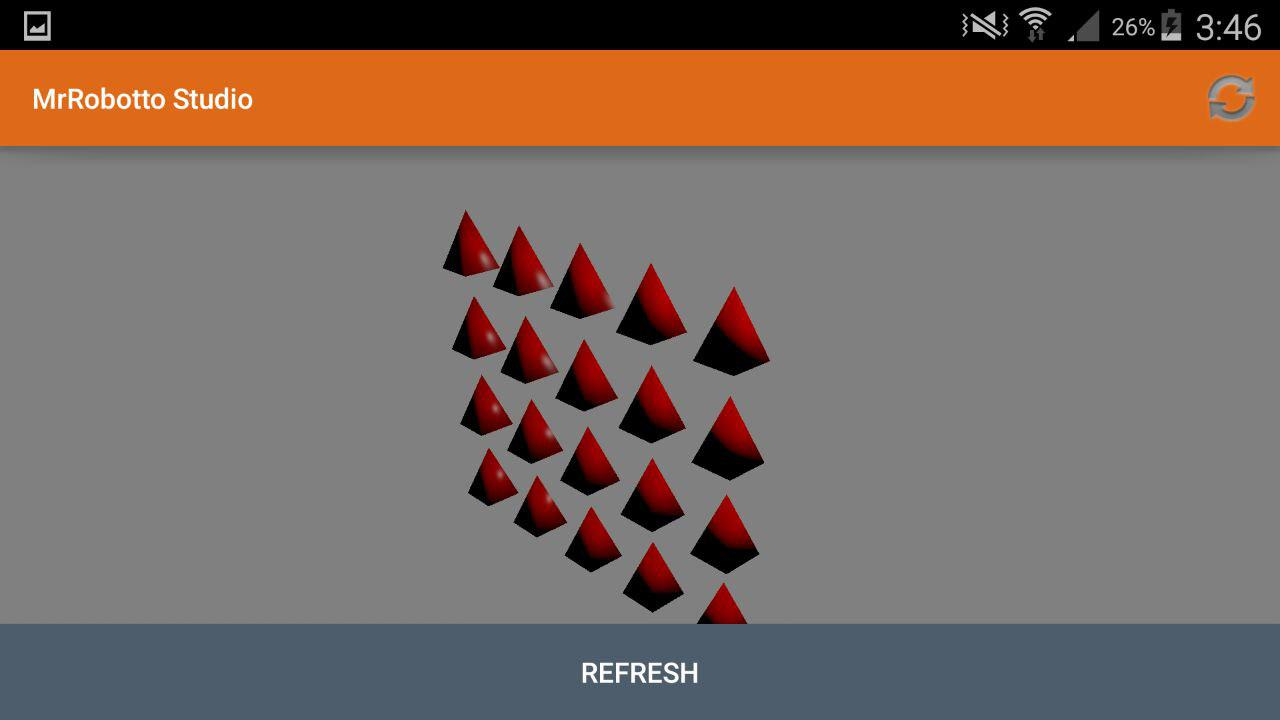
\includegraphics[scale=0.1]{benchmarks/simple/20.jpg}
}
\subfloat[50 objetos]{
  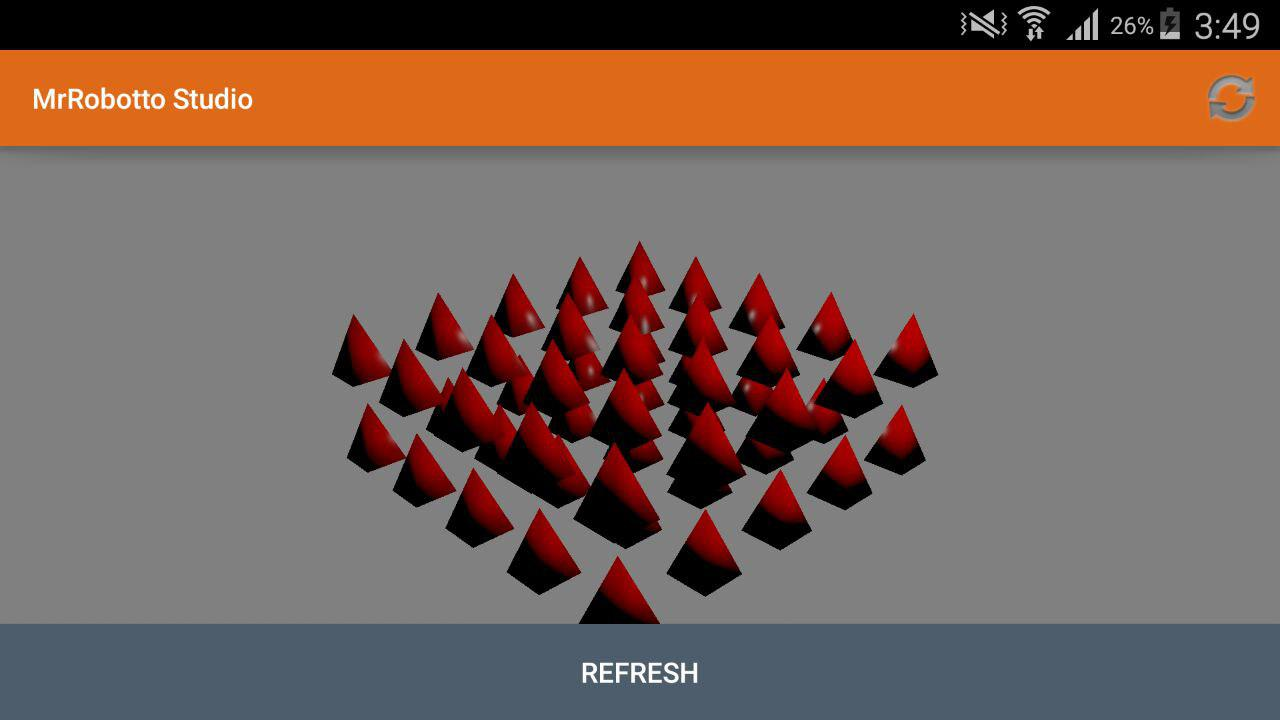
\includegraphics[scale=0.1]{benchmarks/simple/50.jpg}
}
\hspace{0mm}
\subfloat[80 objetos]{
  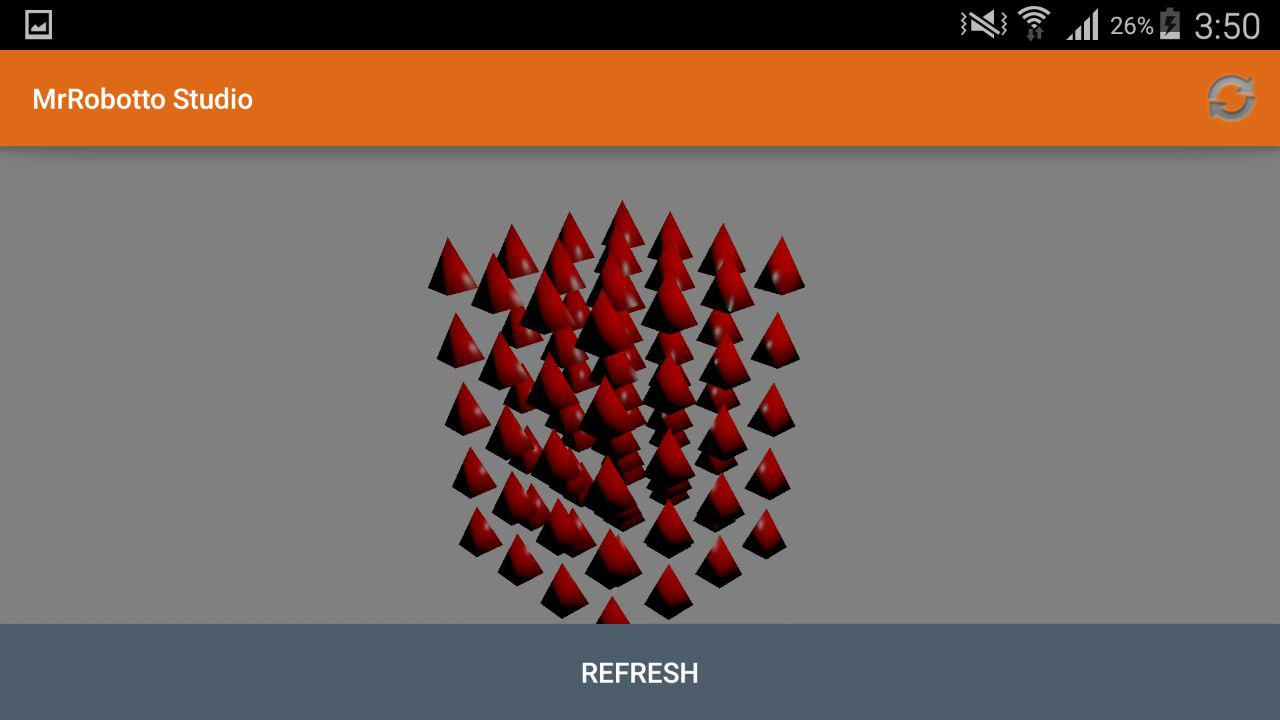
\includegraphics[scale=0.1]{benchmarks/simple/80.jpg}
}
\caption[Renderizado de objetos simples]{Renderizado de objetos simples}
\label{fig:benchmarksimple}
\end{figure}

\subsection{Renderizado de Múltiples Objetos Animados}
TODO: Cuadro con los FPS al renderizar una escena con por ejemplo
5, 20, 50 y 100 modelos realizando una animacion
\subsection{Renderizado de Múltiples Objetos y Múltiples Texturas}
TODO: Cuadro con los FPS al renderizar una escena con por ejemplo
5, 20, 50 y 100 modelos cada uno con textura distinta

